\documentclass[12pt,a4paper]{article}

%-------------------Packages-------------------%
\input Acorn.fd
\usepackage[magyar]{babel}
\usepackage[T1]{fontenc}
\usepackage{kpfonts}
\usepackage{changepage}
\usepackage{xcolor}
\usepackage{tikz}
\usepackage{wrapfig}
\usepackage{hyperref}
\usepackage{fancyhdr}
\pagestyle{fancy}
\usepackage{anyfontsize,lettrine}
\usepackage{pdfpages}

%-------------------Settings-------------------%
\graphicspath{{./images/}}
\setlength\parindent{0pt}


\cfoot{}

\lhead{\rightmark}
\rhead{\thepage}
\setcounter{DefaultLines}{3}
\renewcommand{\LettrineFontHook}{\usefont{U}{Acorn}{xl}{n}}
%-------------------Commands-------------------%
\newcommand{\AUTHOR}{Herőczi Sándor}
\newcommand{\NEPTUN}{WH0AMC}
\newcommand{\TITLE}{Mikrovezérlő alapú autonóm fegyverrendszer tervezése és fejlesztése}
\newcommand{\YEAR}{2024}
\newcommand{\LOCATION}{Budapest}
\newcommand{\ABRAKELL}{\textcolor{red}{IDE KELL MÉG ÁBRA}}
%-------------------Colours-------------------%
\definecolor{BMEbordo}{HTML}{862633}


\newcommand{\w}[1]{\; \mathrm{#1}}
\newcommand{\q}[1]{\; \left[\mathrm{#1}\right]}

\begin{document}

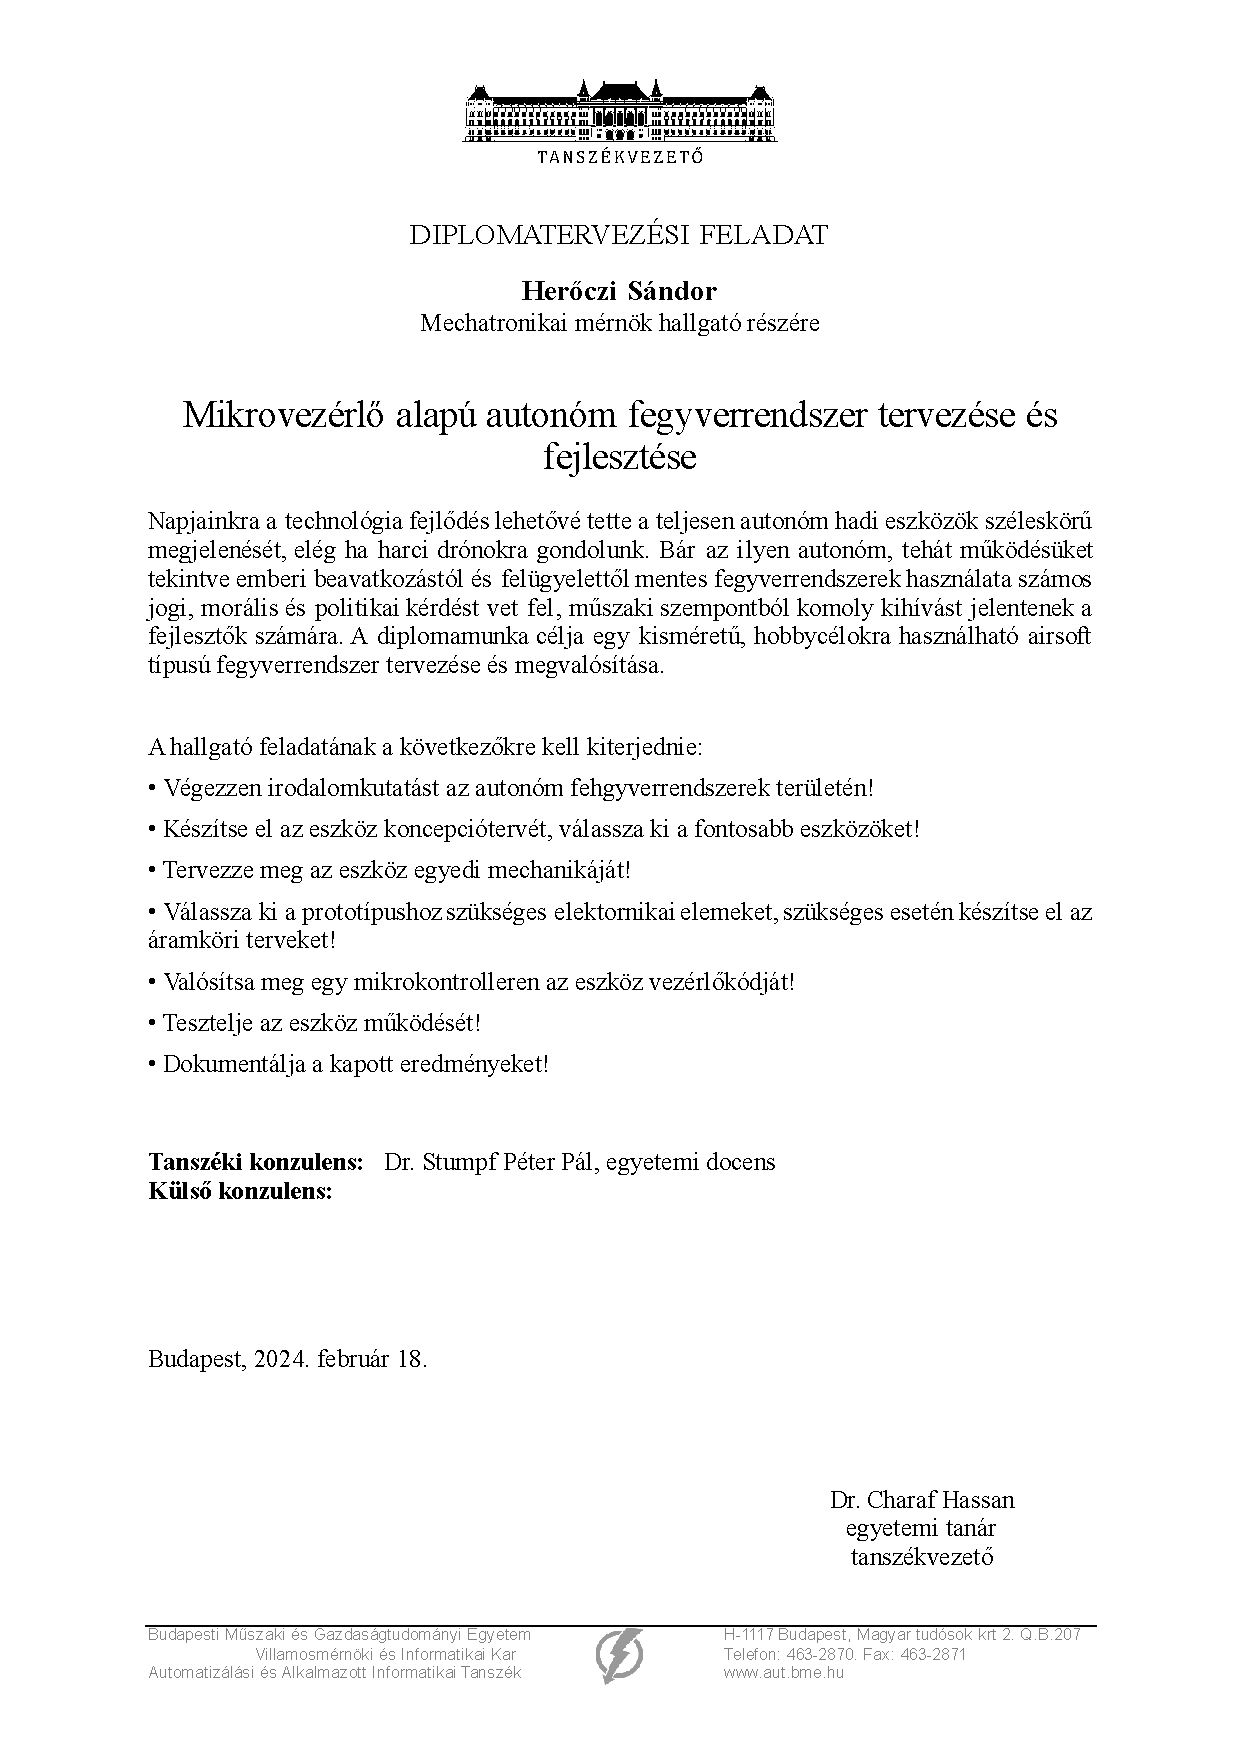
\includepdf[pages=-]{feladatkiiras.pdf}

\begin{titlepage}
	\begin{adjustwidth}{-2.5cm}{-2.5cm}

	
	\thispagestyle{empty}
	\centering

	\Large
	\rule{16cm}{1pt}\\
	\textsc{
		Budapesti Műszaki és Gazdaságtudományi Egyetem\\
		Villamosmérnöki és Informatikai Kar\\
		Automatizálási és Alkalmazott Informatikai Tanszék}\\[-0.3cm]
	\rule{16cm}{1pt}
	\end{adjustwidth}
	
	\vspace{2cm}
	
	\flushleft
	\Huge
	\textbf{\TITLE}
	
	\vspace{3cm}
	
	\Large
	\textbf{\AUTHOR}\\
	\NEPTUN\\
	
	\begin{tikzpicture}[overlay, remember picture]
		\node[anchor=center, xshift=5cm, yshift=-10cm] at (current page.center)
		{
\includegraphics[height=2cm]{autlogo}}; 
	\end{tikzpicture}
\end{titlepage}

\pagebreak

\section*{Hallgatói nyilatkozat}

Alulírott Herőczi Sándor, szigorló hallgató kijelentem, hogy ezt a diplomatervet meg nem engedett segítség nélkül, saját magam készítettem, csak a megadott forrásokat (szakirodalom, eszközök stb.) használtam fel. Minden olyan részt, melyet szó szerint, vagy azonos értelemben, de átfogalmazva más forrásból átvettem, egyértelműen, a forrás megadásával megjelöltem.\\

Hozzájárulok, hogy a jelen munkám alapadatait (szerző(k), cím, angol és magyar nyelvű tartalmi kivonat, készítés éve, konzulens(ek) neve) a BME VIK nyilvánosan hozzáférhető elektronikus formában, a munka teljes szövegét pedig az egyetem belső hálózatán keresztül (vagy hitelesített felhasználók számára) közzétegye. Kijelentem, hogy a benyújtott munka és annak elektronikus verziója megegyezik. Dékáni engedéllyel titkosított diplomatervek esetén a dolgozat szövege csak 3 év eltelte után válik hozzáférhetővé.\\

Kelt: \LOCATION, 2024.06.02.\\

\hfill
\begin{tabular}{c}
	........................................... \\
	Herőczi Sándor \\
\end{tabular}

\pagebreak

\section*{Összefoglaló}
A diplomamunkám célja egy autonóm fegyverrendszer fejlesztése és elkészítése, amely funkciójában hasonlít a valós, éles helyzetben alkalmazott rendszerekhez. Ez annyit takar, hogy a fegyvernek képesnek kell egy bizonyos méretű területet belátni, ebben felismerni és azonosítani a célpontokat, majd tüzelni, vagy engedélyt kérni tüzelésre. Ezentúl szükséges funkciója a manuális vezérlés, amely segítségével az operátor valós időben tudja távolról irányítani az eszközt, egy asztali számítógép segítségével.\\

Az eszköz alkatrészei 3D nyomtatási technológiával készültek, a kötőelemeket, csapágyakat és elektronikai elemeket kivéve, első feladatom ezek nyomtatáshelyes megtervezése volt. A következő lépés a hardver és elektronikai rendszer tervezése volt, majd a szükséges modulok, szenzorok, mikrovezérlő kiválasztása és megrendelése. Az utolsó alfeladat pedig a szoftver fejlesztése, amely jelentette mind a beágyazott vezérlő szoftvert, és a számítógépen futó felhasználói felületet is.\\

A projekt megvalósítása során végig sok időt emésztett fel a rendszer tesztelése, amelyet párhuzamosan kellett végezni a későbbi alfeladatok tervezésével. Kihívást jelentett a megfelelően részletes szakirodalom felkutatása is, ugyanis a valós megoldások paramétereit gyakran nem teszik elérhetővé civilek számára, illetve a jelenleg folyó fejlesztések is titkosítottak.\\

Úgy gondolom, a téma interdiszciplináris jellegét tekintve jól illik a mechatronikai tanulmányaiba, ugyanis egyaránt érinti a műszaki mechanika,  a gyártástechnológia, a szoftverkészítés és a jelfeldolgozás területeit.\\

Diplomamunkám eredményeként megvalósítok egy működő prototípust, amit előadás keretében fogok bemutatni. Végül pedig kitérek az esetleges hibákra amiket elkövettem, a tanulságokra és a továbbfejlesztési lehetőségekre.

\pagebreak

\section*{Abstract}
The aim of my thesis is to develop and build an autonomous weapon system that functions similarly to real-world systems used in live scenarios. This means that the weapon must be able to monitor a designated area, recognize and identify targets, then fire or request permission to fire. Additionally, a necessary feature is manual control, allowing the operator to remotely control the device in real-time using a desktop computer.\\

The components of the device were created using 3D printing technology, except for the fasteners, bearings, and electronic elements. My first task was to design these components to be suitable for printing. The next step was to design the hardware and electronic system, followed by selecting and ordering the necessary modules, sensors, and microcontroller. The final subtask was the development of the software, which included both the embedded controller software and the user interface running on a computer.\\

Throughout the project, significant time was consumed by system testing, which had to be carried out simultaneously with the planning of subsequent subtasks. A challenge was also posed by finding sufficiently detailed technical literature, as the parameters of real-world solutions are often not made available to civilians, and current developments are often classified.\\

I believe that the interdisciplinary nature of this topic fits well with my mechatronics studies, as it encompasses areas such as mechanical engineering, manufacturing technology, software development, and signal processing.\\

As a result of my thesis, I will produce a working prototype, which I will present during my final defense. Lastly, I will address any mistakes I made, lessons learned, and possibilities for future development.
\pagebreak

\tableofcontents

\pagebreak

\section{Bevezetés}

\subsection{Motiváció és háttér}

\lettrine{E}zt a projektet nem a tanszéki diplomamunkatémák listáján találtam, hanem én kerestem hozzá konzulest. Szeretném ezért először megemlíteni a személyes motivációmat, és érdekeltségeimet vele kapcsolatban. Mint a legtöbb reál beállítottságú fiú, engem is fiatal korom óta érdekel a technológia, a járművek, a gépek, vagy a fegyverek. Ezek közös metszéspontja a haditechnológia, ami általában jóval fejlettebb, mint amivel a civil életben találkozhatunk. Ez az érdeklődés megmaradt kamaszkoromra is, amikor a videojátékok által új ingerként értek a \textsl{Team Fortress 2}-ben és a \textsl{Portal}-ban lévő ún. \textbf{Sentry Gun}-ok. Ezek olyan lövegek , amelyek a lábukon állva képesek voltak forogni, és ha az ellenség a látóterükbe jutott, akkor arra tüzet nyitottak. Nyilván játékokról van szó, tehát mindig azt hittem hogy ez csak a jövő technológiája, de nem sokkal később rá kellett jönnöm, hogy nagyon is valódiak. Ezután, mikor már egyetemre jártunk, egy barátommal egyre komolyabban kezdtünk beszélgetni arról, hogy esetleg mi is tudnánk egyet építeni. Végül az egyetemi éveim végére érve el is jött a tökéletes alkalom, hogy megvalósítsam régi álmomat. \\

A szentimentalitást félretéve, természetesen nem választottam volna ezt a témát, ha nem lenne a tanulmányaim szempontjából is releváns. Úgy gondolom, ez a projekt a mechatronika oktatás sok fontos elemét magában hordozza. A feladat a mechanikai konstrukcióval kezdődik és a CAD modellezéssel, amely a gépészeti oldalát hasznosítja a képzésünknek. Foglakozni kell a hardverrel, amihez elektronikai ismeretek szükségesek. Végül pedig a szoftvert kell lefejleszteni, ami informatikai szempontból érdekes. Ráadásul az egész beágyazott környezetben történik, ami miatt még relevánsabb az \textsl{intelligens beágyazott rendszerek} specializációmhoz. Véleményem szerint a projekt nehézsége és kihívása nem az egyes alfeladatokban rejlik, hanem az egész rendszer integrálásában, egymáshoz illesztésében. \\

Szintén fontosnak tartom megemlíteni, hogy a feladat lehetőséget ad megismerni és használni pár igen modern technológiát. A közelmúltban elérhetővé (és megfizethetővé) váltak civil felhasználásra a 3D nyomtatók, valamint a fejlődés a \textsl{Deep Learning} algoritmusok terén nagyban befolyásolta a gépi látás szakterületét is. Többek között a célom, hogy jobban megismerkedjek ezekkel a módszerekkel, és alkalmazzam őket.

\pagebreak

Mint manapság az ipar minden területén, így a fegyveriparban is egyre nagyobb mértékű a digitalizáció és az automatizáció. Ennek ékes példája a távolról irányítható lőállások térnyerése, amelyeknek nagy előnye a fegyver és a tüzér egymástól való elkülönítése, aminek több előnye is van. Természetesen a legfontosabb és leginkább szembetűnő, hogy ezzel a módszerrel minimalizálható, vagy akár megszüntethető a saját embereink életének kockáztatása. Ezentúl olyan helyen is tudjuk használni ezeket az eszközöket, ahova egy tradicionális géppuskafészek telepítése nehézkes lenne, például mostoha természeti körülmények közé, egy torony tetejére, vagy akár egy hadihajó oldalára. Szintén egy nagy előny, hogy ezek az eszközök felszerelhetők több kezeléssegítő alegységgel, például hőkamerával vagy éjjellátóval. Majdnem minden, számottevő hadsereggel rendelkező országnak van saját fejlesztésű távirányított fegyverrendszere.\\


\begin{wrapfigure}{r}{0.45\textwidth}
	\centering
	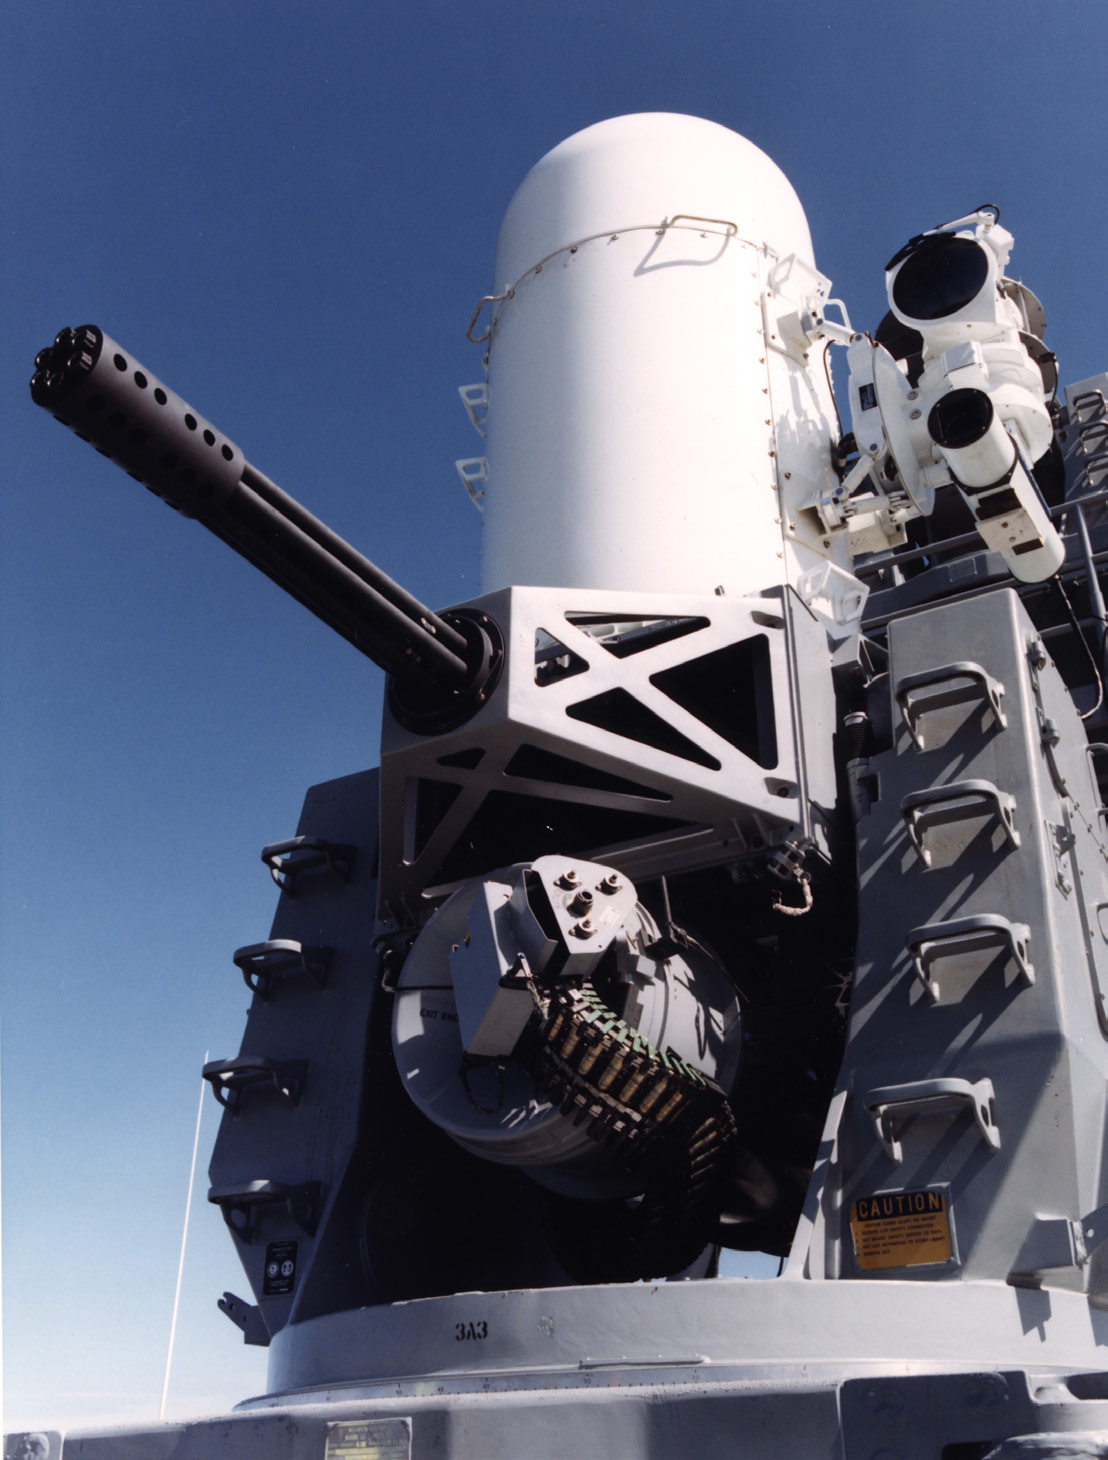
\includegraphics[width=0.95\linewidth]{irod_phalanx} 
	\caption{Phalanx CIWS rendszer}
	\label{fig:irod_phalanx}
\end{wrapfigure}

A következő lépés az automatizálás. Hiszen egyre erősebb hardverekkel rendelkezünk, egyre jobb algoritmusokat tudunk implementálni, és elértük az a szintet, hogy bizonyos helyzetekben a "gép" jobb munkát tud végezni, mint egy ember. Az első automatikus célzórendszerrel rendelkező légvédelmi gépágyú az amerikai \textsl{Phalanx CIWS} az 1970-es években került kifejlesztésre, ezzel megszületett a "Lethal autonomous weapon (LAW)" kifejezés.\\

A technológiát érthető módon leggyakrabban védelmi célokra használják, sokszor légvédelemre. A gyakorlatban nagy szerepe van Dél-Korea és Izrael védelmében, ahol a rakétatámadások mindennapos veszélyt jelentenek. Offenzív célokra a gyakorlatban még csak rakéták célzására használnak automatikát, a "terminátor" jellegű gyilkos robotok még csak fejlesztési fázisban vannak.
\pagebreak 

\subsection{Kihívások és célkitűzések}

A hagyományos, ember által irányított biztonsági rendszerek, illetve manuálisan vezérelt fegyverek hatékonysága korlátozott. Az ember reakcióideje lassú lehet krízishelyzetben, különösen ha nagy sebességű, gyors reagálású, esetleg automatizált a célpont. További gyengesége az embernek, hogy hajlamos hibázni. A fáradtság, stressz, éhség, és rengeteg egyéb tényező kényszerítheti hibára. Ez szükségessé teszi egy olyan automata rendszer kifejlesztését, amely képes azonnal reagálni, felismerni a fenyegetéseket és pontosan célozni.\\

Az automatikus gépágyúk fejlesztése során számos technikai kihívás merül fel:

\begin{list}{}{}
	\item \textbf{Célpontok felismerése és követése:} A gépágyúnak gyorsan és pontosan kell érzékelnie és nyomon követnie mozgó célpontokat. Ez kihívást jelenthet változó fényviszonyok, mozgássebességek és környezeti zavaró tényezők mellett. A gépágyúnak gyorsan és pontosan kell érzékelnie és nyomon követnie mozgó célpontokat. Ez kihívást jelenthet változó fényviszonyok, mozgássebességek és környezeti zavaró tényezők mellett. \\
	\item \textbf{Pontosság és reakcióidő:} A rendszernek gyorsan kell döntéseket hoznia, ugyanakkor elengedhetetlen a pontos célzás. A mechanikai mozgásvezérlés, a számítógépes látás és az elektronikai rendszerek szinkronizációja mind kritikus tényező a rendszer hatékonysága szempontjából. \\
	\item \textbf{Környezetérzékenység:} Külső környezeti tényezők (pl. időjárás, akadályok, fényviszonyok) befolyásolhatják a rendszer működését, ezért a szoftvernek és a hardvernek rugalmasnak és robusztusnak kell lennie. 
\end{list}
A dolgozatom célja egy innovatív megoldás kidolgozása, amely eleget tesz a megszabott követelményeknek és megoldást nyújt a fenti problémákra. \\

\pagebreak

Kiemelt célok:
\begin{list}{}{}
	\item Egy megbízható célpontfelismerési rendszer fejlesztése, amely változó környezeti feltételek mellett is képes hatékonyan működni.
	\item Egy stabil és erős mechanikai konstrukció tervezése, amely képes képes követni a szoftver utasításait.
	\item Egy olyan valós idejű szoftvervezérlési rendszer megalkotása, amely gyorsan reagál a célpontok mozgására és változására.
\end{list}

Összegezve \textbf{Egy olyan automata gépágyú fejlesztése és megépítése, amely magabiztosan képes felismerni egy célpontot, követni azt, célozni, és tüzelni.}

\subsection{Korlátozások}

Természetesen tisztában kell lenni bizonyos korlátozásokkal a projekt elkészítése közben. Két félévem van lefejleszteni az eszközt a nulláról, egyedül vagyok, és nincsen százmilliós büdzsém, mint az iparban hasonló kutatással foglalkozó csapatoknak. Ebből kifolyólag reálisan kell látni a helyzetet, és úgy meghatározni a követelményeket, hogy egy egyetemi hallgató számára is elérhető legyen. \\

A kamerarendszer például, amit a valós megoldásokban használnak, önmagában tízmilliós tétel szokott lenni. Sajnos az én megvalósításom valószínűleg nem fog működni sötétben, nagy távolságokban, vagy esőben, hiszen a költségvetésbe nem fér bele az éjjellátó, a hőkamera, az optikai zoom vagy több kamerából álló rendszer.\\

Nem áll rendelkezésemre korlátlanul se CNC gép, se fém 3D nyomtató, így a legtöbb alkatrész műanyagból kell 3D nyomtatnom. Ez befolyásolhatja a szerkezet stabilitását, amit figyelembe kell venni a későbbiekben.\\

És végül fontos megemlíteni, hogy mivel éles fegyvert alkalmazni minden bizonnyal a törvénybe ütközne, ezért valamilyen játékfegyvert kell majd használnom. Ez befolyásolni fogja a gépágyú pontosságát, amit szintén figyelembe kell venni a tervezéskor és értékeléskor.\\


\pagebreak

\subsection{Erkölcsi nyilatkozat}
Az automata fegyverrendszer morális megítélése vitatott téma, ezért szeretném kijelenteni, hogy diplomamunkám, melynek címe \textsl{„Mikrovezérlő alapú autonóm fegyverrendszer tervezése és fejlesztése”}, kizárólag tanulányni és mérnöki célokat szolgál. A dolgozatom keretében fejlesztett prototípus semmilyen formában nem szándékozik vagy ösztönzi az erőszakos, káros vagy törvénysértő tevékenységeket. Fejlesztésem célja a technológiai kutatás, a mechatronikai és automatizálási rendszerek megismerése, illetve a gépi látás alkalmazásainak tanulmányozása. \\

Határozottan elhatárolódom bármilyen rosszindulatú felhasználástól, és hangsúlyozom, hogy a projekt eredményei nem használhatók fel ártalmas vagy illegális célokra. A munka során mindvégig tiszteletben tartottam az etikai irányelveket, és felelős mérnöki magatartást tanúsítottam. Az általam fejlesztett rendszer kizárólag oktatási, kutatási és technológiai demonstráció célját szolgálja.

\pagebreak


\section{Irodalomkutatás}
A legjelentősebb katonai hatalmak mindegyike rendelkezik távvezérelt fegyverrendszerekkel, leggyakrabban valamilyen távolról irányított gépfegyver formájában. Azonban se az egyes országok nemzetbiztonságának, se a fegyveripari partnercégeknek nem áll érdekében a szükségesnél több információt kiadni. Ez egy kicsit megnehezítette az irodalomkutatást, de a képek alapján azért sok információt ki lehet nyerni.

\subsection{Megvalósult rendszerek} \label{sec:valos}

\paragraph{CROWS \cite{crows}}
Az egyik legnagyobb darabszámban gyártott távirányított fegyverrendszer az amerikai \textsl{CROWS} rendszer, amely a NATO-országokban, köztük Magyarországon is rendszeresített. Ennek értelmében telepíthető sok NATO által használt páncélozott járműre, köztük a Humvee-ra, a Stryker-re, és a Buffalo MRAP-re. Több verziója létezik több kaliberrel, a \ref{fig:irod_crows}. ábrán egy M240B géppuskával látható.\\

\begin{figure}[h!]
	\centering
	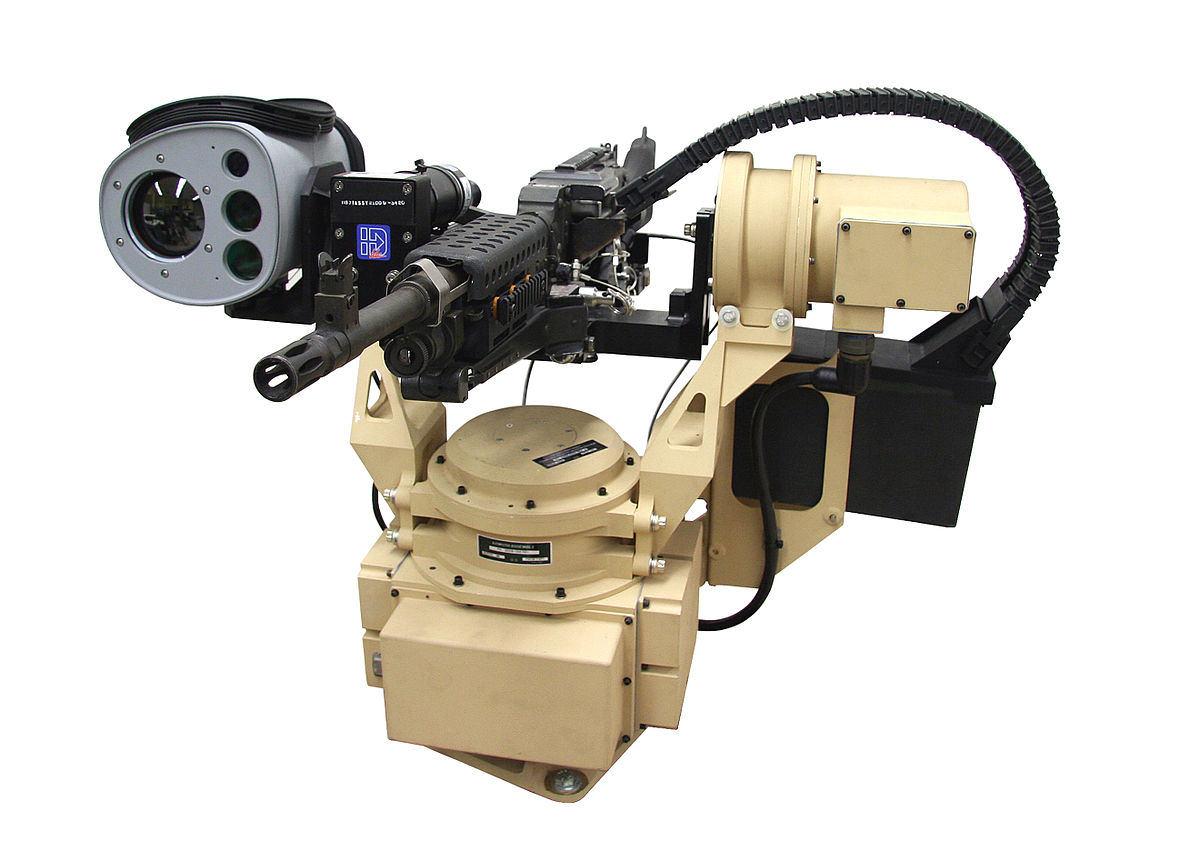
\includegraphics[width=1\linewidth]{irod_crows}
	\caption{Az amerikai CROWS rendszer}
	\label{fig:irod_crows}
\end{figure}

A szerelék a fegyverrel együtt $360^\circ$-ban képes elfordulni, és $-20^{\circ}$-tól $+60^{\circ}$-ig tud billenni. A fegyvercső giroszkóppal stabilizált. A kezelő egy 15 hüvelykes kijelzőn tud célozni a fegyverrel. A rendszer a sima kamera mellett rendelkezik hőkamerával is, így éjszaka is használható. Mind a két kamera el van látva lézeres távolságmérővel, amivel rá lehet állni a célpontra, és a jármű mozgása közben is lehet azt követni. A kamerát és a fegyvert lehet külön is mozgatni, ami azért hasznos, mert anélkül lehet követni a gyanús alakok mozgását, hogy félelmet keltenénk az emberekben.

\paragraph{Arbalet-DM \cite{arbalet}}
A \textsl{CROWS} rendszer orosz megfelelője a hasonló kialakítású \textsl{Arbalet-DM} (\ref{fig:irod_arbalet}.ábra). Ennek a rendszernek az alapja a 12.7 mm-es KORD nehézgéppuska. Rendelkezik 4 gránátvetővel is, amelyek füstfüggöny felhúzására használható. A kamera és a fegyver elhelyezése, de még a lőszer pozíciója is teljesen hasonló az amerikai párjához.

\begin{figure}[h!]
	\centering
	\includegraphics[width=1\linewidth]{irod_arbalet}
	\caption{Az orosz Arbalet-DM rendszer}
	\label{fig:irod_arbalet}
\end{figure}

A rendszer $360^\circ$-ban képes elfordulni, és $-20^{\circ}$-tól $+70^{\circ}$-ig tud billenni, tehát egy kicsit nagyobb részt tud lefedni, mint a CROWS. A hatótáv nappal 2000 m, éjszaka 1500 m. Ez a rendszer is el van látva hőkamerával és lézeres távolságmérővel.

\paragraph{DeFNder \cite{defnder}}
A következő megoldás a belga \textsl{DeFNder} termékcsalád, amelynek két tagja a \textsl{Light} és a \textsl{Medium}(\ref{fig:irod_defnder}. ábra). Értelem szerűen kettő közül az utóbbi az, amelyre nehezebb fegyverzetet lehet telepíteni. A függőleges tengelyen $360^\circ$-ban képes elfordulni 90 fok/másodperc sebességgel, a vízszintes tengelyen $-45^{\circ}$-tól $+75^{\circ}$-ig tud billenni, 60 fok/másodperc sebességgel. Opcionálisan ellátható infravörös- és hőkamerával a rossz látási körülmények esetére, valamint lézeres távolságmérővel a ballisztikai kompenzációhoz.
\begin{figure}[h!]
	\centering
	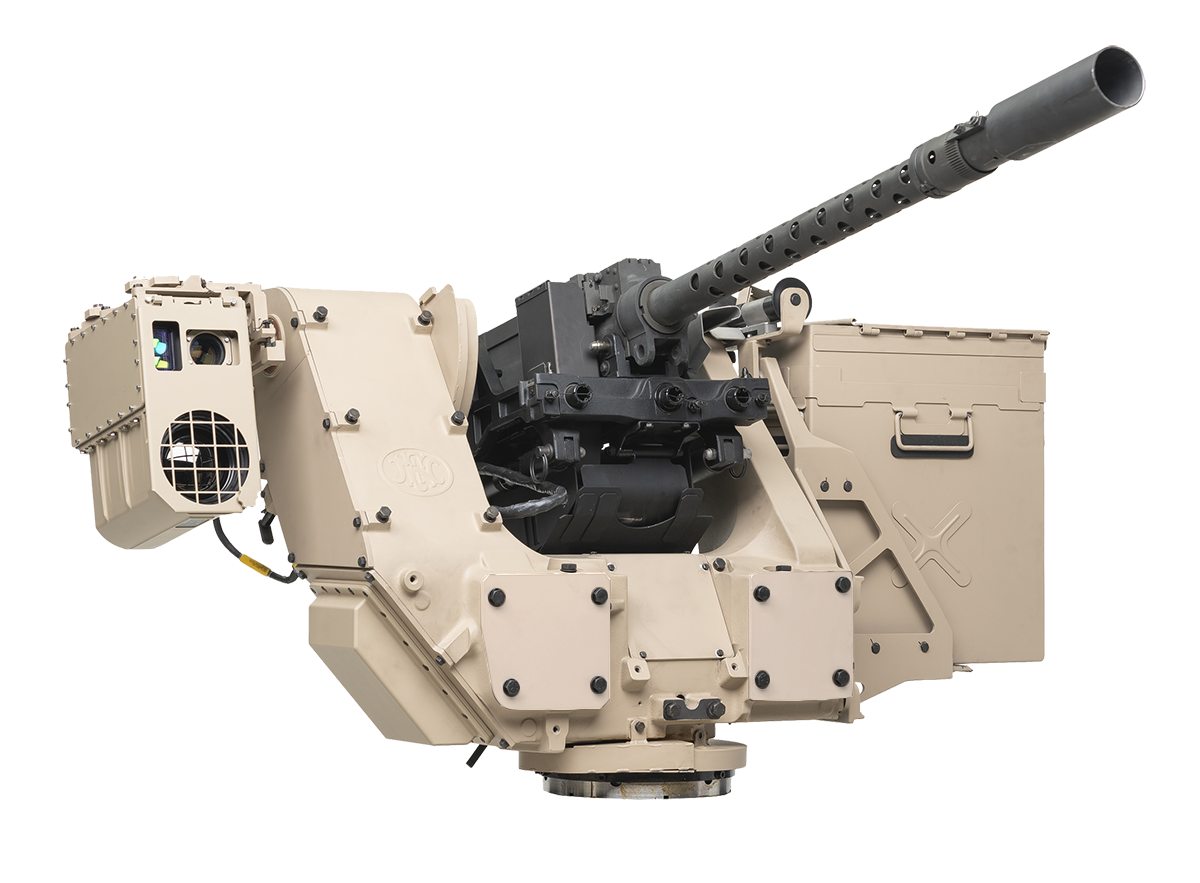
\includegraphics[width=1\linewidth]{irod_defnder}
	\caption{A belga DeFNder rendszer}
	\label{fig:irod_defnder}
\end{figure}

Elég sok közös vonást találtam a fentebb említett rendszerekben. Az elrendezésük nagyon hasonló, van egy függőleges forgástengely nagyjából a teljes rendszer súlypontján keresztül, valamint egy vízszintes forgástengely, nagyjából a fegyver csövével egy síkban. Erre valószínűleg azért van szükség, hogy a tüzelés során keletkező erők ne ébresszenek csavarónyomatékot a mozgató mechanizmuson. Az én esetemben nagy erők nem fognak ébredni, de a tervezési elvet érdemes követni.

\paragraph{Samsung SGR-A1}
Az egyetlen, valós harci helyzetben használt, teljesen autonóm gépágyú a koreai fejlesztésű \textsl{Samsung SGR-A1}. A két Korea között húzódó demilitarizált övezet (DMZ) egy 250 km hosszú, 4 km széles sáv, amelyet mind a két oldalon szigorúan ellenőriznek. A határ folyamatos felügyelete rengeteg ember munkájába kerül, ami egy demográfiai válságban lévő ország csökkenő hadseregében egyre értékesebb. Főleg annak tekintetében, hogy csupán járőrözni és figyelni a határt nem feltétlenül igényli egy ember jelenlétét. Ennek tudatában fejlesztették ki a Samsung és a Korea Egyetem mérnökei az SGR-A1 fegyverrendszert. Hőkamerával és éjjellátóval felszerelve napközben 4 km-ről, éjszaka 2 km-ről képes azonosítani potenciális célpontokat, tehát tulajdonképpen a DMZ teljes szélességében. Képes felismerni az embereket, követni őket, és megkülönböztetni az állatoktól. Hangfelismeréssel képes azonosítani a közeledő személyeket: amennyiben valaki 10 m-nél közelebb kerül és nem azonosítja magát, a rendszer riaszthat, gumilövedéket lőhet, vagy használhatja a K-3 gépfegyverét.

\begin{figure}[h!]
	\centering
	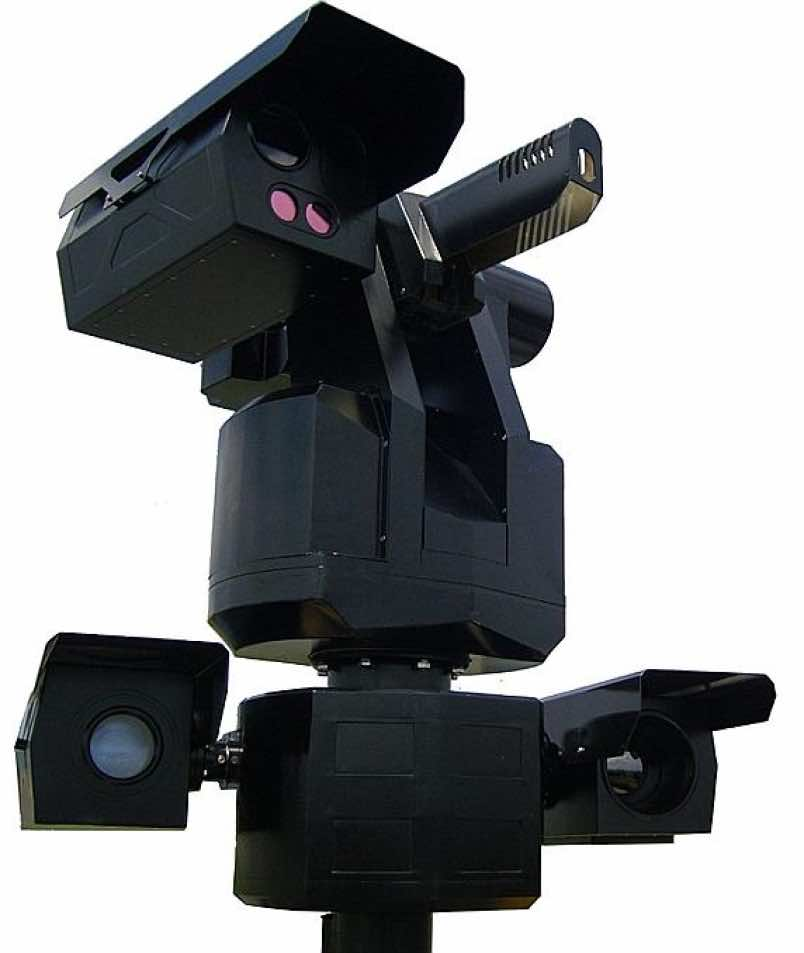
\includegraphics[width=0.5\linewidth]{irod_samsung}
	\caption{Samsung SGR-A1}
	\label{fig:irod_samsung}
\end{figure}

Sok szakértő találgatja, hogy a rendszer lőhet-e emberi engedély nélkül, és a hivatalos koreai álláspont az, hogy nem. Azonban ha már bemérte és ellenségként azonosította a célpontot, akkor nehéz elképzelni, hogy pont a ravaszt ne tudná meghúzni.

\pagebreak

\subsection{Tüzelési mechanizmus}

A korábban említett rendszerek éles fegyverekkel vannak felszerelve, ami az én esetemben sajnos nem megvalósítható. Így valamilyen más megoldást kellett találni, ami legális, és megfelelően be lehet vele mutatni a célfelismerés és célzás működését. 


\paragraph{Paintball}

Több, a diplomamunkámhoz hasonló projektet is találtam, amelyek paintball puskákat használnak. Ezek a puskák sűrített levegőt alkalmaznak, hogy egy festékkel töltött golyót lőjenek ki. A torkolati sebességük nagyjából 280 fps, maximális hatékony távolságuk kb 25-30 m. Mivel a lövedék alakja gömb, és a cső sincs huzagolva, ezért nem túl pontos, főleg hosszú távon.\\

\begin{figure}[h!]
	\centering
	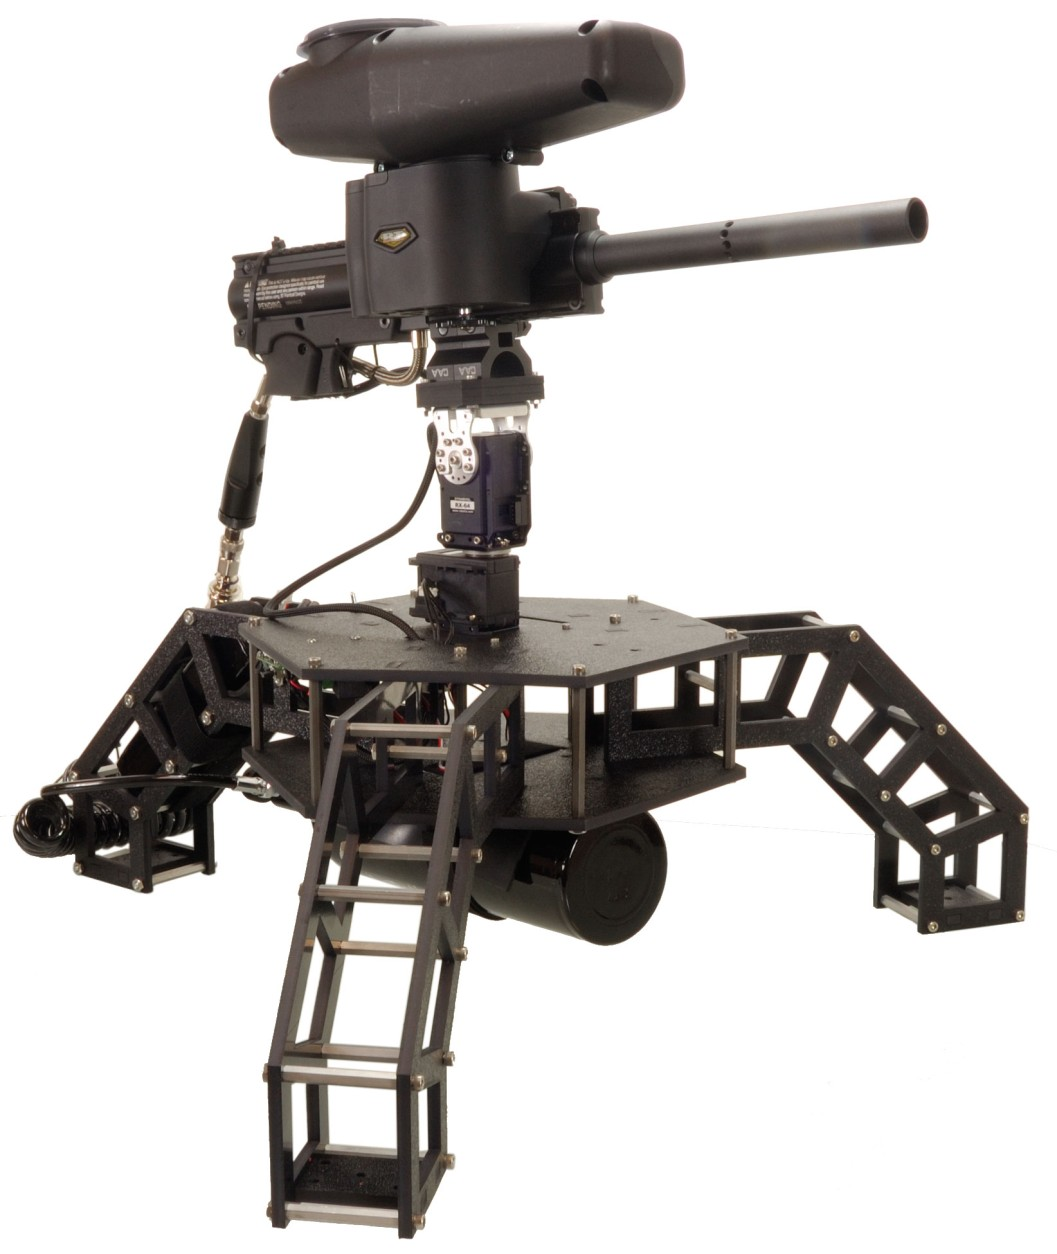
\includegraphics[width=0.6\linewidth]{irod_paintball}
	\caption{Paintball puska alapú rendszer}
	\label{fig:irod_paintball}
\end{figure}

További problémák, hogy a legolcsóbb paintball puska is 70000 Ft. fölött van, valamint a lövedék is viszonylag drága, és nem lehet újrahasznosítani. Ezentúl a fegyverek nagyok, nehezek, és ezért nehéz a beépítésük. 


\paragraph{Nerf}

A Nerf fegyverek a legelterjedtebb játékfegyverek. Sűrített levegővel lőnek ki egy hosszúkás szivacs lövedéket. A sűrített levegőt egy megfeszített rugó elengedésével érik el, amelyet vagy kézzel, vagy valamilyen áttételes villanymotorral húznak fel. A legjobb modellek torkolati sebessége 70 fps körül van, és kb. 15 m a hatótávolságuk. Ezen a távon viszonylag pontosak a lövedék kialakításából adódóan, de jelentős az esés, így a ballisztikai pályát komolyan kell venni. \\

Ezek a fegyverek modelltől függően 10000 Ft. - 40000 Ft. között mozognak, de a lövedékeket újra lehet használni. Az a probléma itt is fennáll, hogy nagy a fegyver teste, így nehezebb beépíteni. 

\paragraph{Airsoft}

Az airsoft fegyverek hasonló módon működnek, mint a Nerf puskák, de egy kisebb, műanyag golyót lőnek. Az elektromos airsoft fegyverek torkolati sebessége általában 300 fps és 400 fps között van, ami befolyásol a golyók tömege, a rugó minősége és rengeteg egyéb alkatrész. A hatótávjuk az átlagos fegyvereknek kb. 50 m, de fejlesztésekkel elérheti a 90 m-t is. A lövedék itt is golyó és a cső sincs huzagolva, mint a paintballnál, azonban az airsoft esetében használnak ún. hop-up kamrákat, amelyek perdületet adnak a golyónak.\\

Az airsoft fegyverek legnagyobb előnye a többi lehetőséggel szemben, hogy van egy kompakt egység, a "gearbox", ami felelős az elsütésért. Ezt ki lehet szedni egy fegyverből, vagy akár külön is meg lehet venni. Ez okkal nagyobb szabadságot ad a beépítéshez, és a végeredmény is sokkal kompaktabb lesz. Az elsütés is csak az áramkör zárását jelenti a gearboxban, ami egyszerűen vezérelhető a mikrokontrollerrel.
\pagebreak

\section{Rendszertervezés és követelmények}
\subsection{Rendszeráttekintés}
Az autonóm fegyverrendszer fejlesztése során egy komplex mechatronikai rendszert kellett megvalósítani, amely több különálló modul együttműködését biztosítja. A rendszer fő komponensei közé tartozik a mechanikai szerkezet, az elektronikai hardver, az érzékelők, a vezérlő egység, valamint a szoftveres háttér. Ezek együttesen biztosítják a rendszer autonóm és manuális működését. Az alábbiakban részletes áttekintést adok a rendszer főbb elemeiről és azok feladatáról.

\subsubsection*{Mechanikai konstrukció}

A váz gyanánt tulajdonképpen egy kéttengelyes pan-tilt mechanizmust kellett megvalósítanom, ami felelős a fegyver stabilan tartásáért és precíz mozgásáért. A váz építőelemei zömében 3D nyomtatási technológiával készültek, ami lehetővé tette a problémák gyors kiküszöbölését, illetve a nagyfokú szabadságot a tervezés során. Ahol tudtam, kereskedelemből beszerezhető alkatrészeket használtam, például a csapágyakat és a kötőelemeket.

\subsubsection*{Elektronikai rendszer}

Az elektronikai rendszer két fő eleme a Raspberry PI, illetve a gearbox volt. Mivel a gearbox igen nagy áramot képes felvenni, külön tápegységgel kellett ellátnom a mikrovezérlőt illetve a golyó kilövéséért felelős elektronikát. A motorok vezérléséért egy kereskedelemben kapható, Raspberryvel kompatibilis shieldet használtam, amely jelentősen megkönnyítette a NEMA-17 típusú léptetőmotorok csatlakoztatását. A lézer diódát és szükséges szenzorokat a Raspberry PI GPIO lábairól vezéreltem, ahogy a gearbox aktiválásáért felelős relét is. A kamera modul egy Raspberry PI Camera V2 volt, amit a mikrovezérlőn található foglalaton keresztül tudtam elérni.

\subsubsection*{Számítógépes vezérlés és szoftveres háttér}

A szoftverfejlesztés során két fő területet kellett lefedni: a vezérlőszoftvert, amely a mikrokontrolleren fut, és az asztali alkalmazást, amely a felhasználói felületet és a magas szintű irányítást biztosítja. A beágyazott vezérlő szoftver felelős a léptetőmotorok mozgatásáért, valamint a szenzorokból érkező információ feldolgozásáért. A számítógépen futó szoftver feladata a felhasználó parancsainak feldolgozása és továbbküldése, valamint a kamera képének megjelenítése valós időben. Mivel a feladat összetett, mind a PC, mind a Raspberry Pi oldaláról történik küldés és fogadás is, ezért több szálon fut egyszerre a szoftver. A két egység közötti kommunikáció során kulcsfontosságú a megfelelő sebesség, ezért a vezetékes kapcsolat mellet döntöttem.

\subsection{Követelmények}\label{sec:kov}

%A követelményeket egyrészt a később említett irodalomkutatás, másrészt pedig a saját ötleteim és a konzulensemmel való egyeztetés alapján alakítottam ki. Az "autonóm fegyverrendszer" alatt én egy olyan eszközt értek, ami egy pontban elhelyezve képes a környezetében felismerni a betanított célpontot, és arra tüzelni. Erre jó fikciós példa a \textsl{Portal} című játékban található \textsl{Sentry turret}, amely a \ref{portalsentry}. ábrán látható. Természetesen a konstrukciós tervezéshez nem ezt vettem alapul, de a működési elvhez adhat jó ötleteket akkor is, ha csak fikció. \\
%
%\begin{wrapfigure}{r}{0.45\textwidth}
%	\centering
%	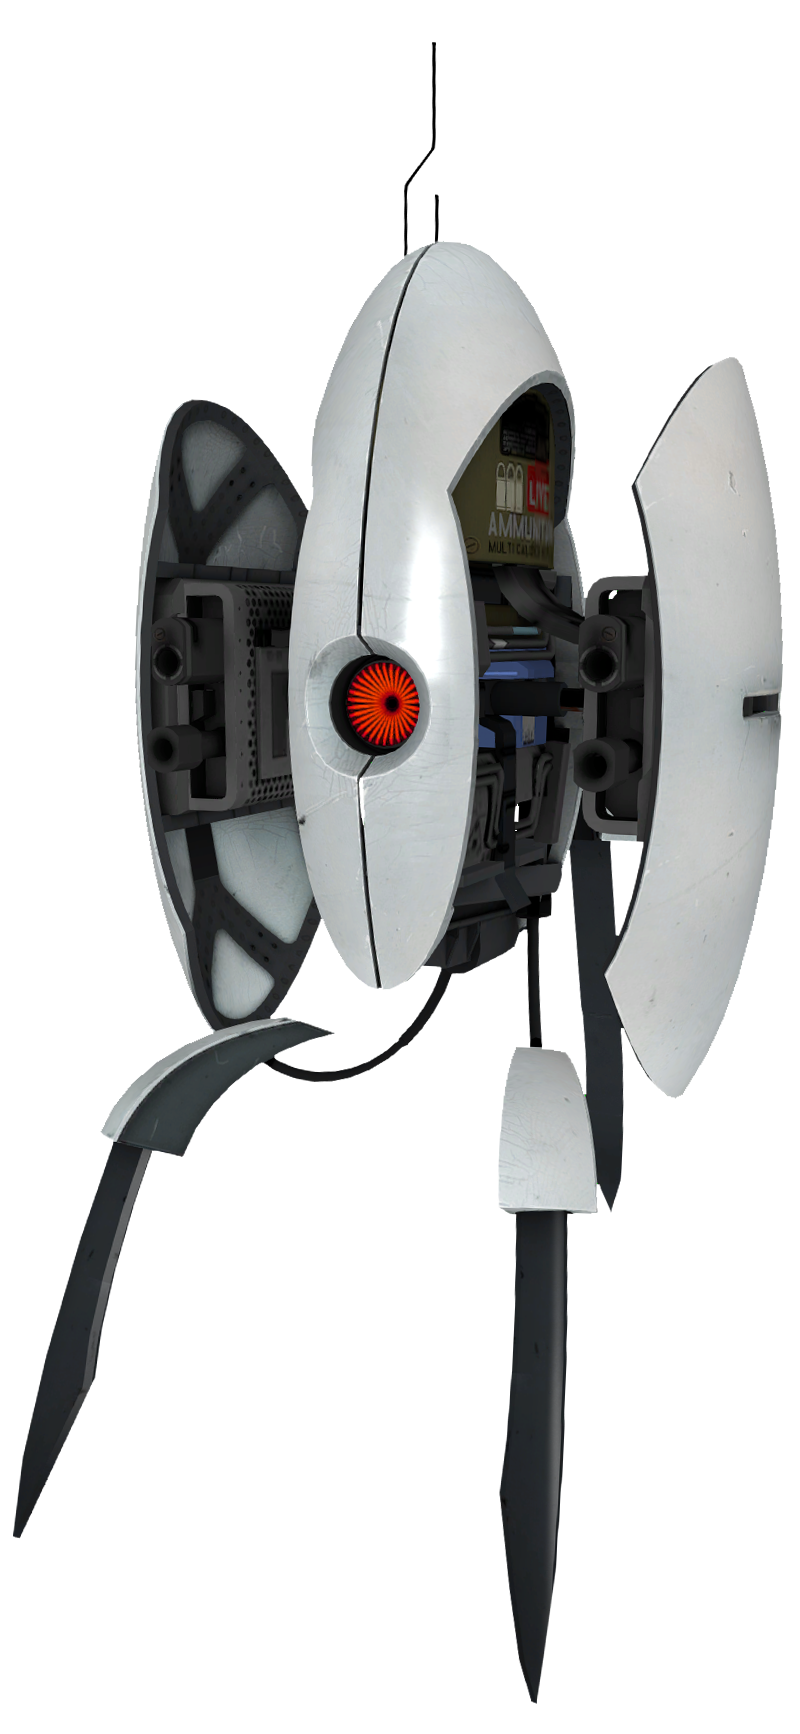
\includegraphics[width=0.8\linewidth]{portalsentry}
%	\caption{Sentry Turret}
%	\label{portalsentry}
%\end{wrapfigure}
%
%Szeretném a rendszert úgy megvalósítani, hogy a célfelismerés és tüzelést lehessen vezérelni "kézi vezérléssel", ahogy a valós katonai rendszerek többsége működik, illetve egy teljesen automatikus gépi látás algoritmussal. Automata működés során is talán az lenne a legéletszerűbb, hogy a célpont megtalálása és becélzása lenne automatikus, a tüzelés pedig emberi engedélyezést igényel, ezzel egy fokkal morálisabbá téve a projektet.\\
%
%A hatásos távolságot én 10m-ben határoztam meg. Ezen a távolságon fel kell ismernie és el kell találnia egy 30x30 cm-es célpontot. Ezentúl szeretném, ha le tudná követni a 10 km/h-val futó ember mozgását. Ezek a határértékek a konstrukció tervezésénél fontos szempontok lesznek, tehát a későbbi fejezetekben számolok velük.\\
%
%\pagebreak

Az autonóm fegyverrendszer fejlesztése során számos követelményt kellett figyelembe venni annak érdekében, hogy a rendszer megbízhatóan, hatékonyan és biztonságosan működjön. Ezek a követelmények a rendszer mechanikai, elektronikai és szoftveres elemeire egyaránt kiterjedtek. A következő szakaszokban részletezem a legfontosabb műszaki és funkcionális követelményeket.

\subsubsection*{Mechanikai követelmények} 

A mechanikai komponensek tervezése során az alábbi követelményeknek kellett megfelelni:
\begin{description}
	\item[Stabilitás és pontosság:]  A fegyverrendszer mechanikai szerkezetének stabilnak és tartósnak kell lennie annak érdekében, hogy a lövések közben ne mozduljon el, és ne veszítse el a célpontot. Ugyanakkor elegendő pontosságot kell biztosítania a célpont precíz követéséhez.
	\item[Fürgeség:]A rendszernek képesnek kell lennie a fegyver gyors és pontos mozgatására a pan-tilt mechanizmus segítségével. Ennek megfelelően a szervomotoroknak kellően gyorsnak és erősnek kell lenniük ahhoz, hogy valós időben tudják követni a mozgó célpontokat.
	\item[Strapabíró konstrukció:] Habár nagy terhelés nem fogja érni, a gearboxból jöhetnek rezgések, rángások, amik esetleg problémát jelenthetnek egy alulméretezett alkatrész esetében.
\end{description}

\subsubsection*{Elektronikai követelmények}

Az elektronikai rendszer megbízható működése érdekében az alábbi követelményeknek kellett eleget tenni:

\begin{description}
	\item[Megfelelő teljesítmény:]  A szervomotoroknak és szenzoroknak megfelelő tápegységre van szükségük, amely stabil energiaellátást biztosít. A rendszer energiaigényét előzetesen fel kellett mérni, hogy a tápegység terhelés alatt is megfelelően működjön.
	\item[Szenzorok pontossága:] A kamerának és egyéb szenzoroknak elegendő felbontással és érzékenységgel kell rendelkezniük ahhoz, hogy képesek legyenek a célpontokat megfelelően azonosítani. A valós idejű képfeldolgozás nagy adatsebességet és megbízható szenzorjeleket igényel.
	\item[Vezérlés:] A mikrokontrollernek kellően gyorsnak kell lennie, hogy a valós idejű adatokat folyamatosan feldolgozza és a vezérlési parancsokat késlekedés nélkül végrehajtsa.
\end{description}


\subsubsection*{Szoftveres követelmények}

A rendszer működéséhez szükséges szoftverfejlesztés során a következő követelményeknek kellett megfelelni:

\begin{description}
	\item[Valós idejű feldolgozás:]  A számítógépes látás szoftverének valós időben kell elemeznie a kamerák által közvetített adatokat, felismerve a célpontokat és kiszámítva a mozgás irányát. A célzási és lövési döntések gyors és hatékony adatfeldolgozást igényelnek.
	\item[Biztonságos működés:] A rendszernek rendelkeznie kell olyan szoftveres biztonsági funkciókkal, amelyek megakadályozzák a véletlen tüzelést. Ez magában foglalja a lövési engedélykérés mechanizmusát és a manuális vészleállítás lehetőségét.
	\item[Felhasználói interfész:] Az felhasználónak egyszerű és intuitív felhasználói felületet kellett biztosítani, amelyen keresztül könnyedén vezérelheti a rendszert, illetve áttekintheti a célpontok adatait és a kamera képét. A felületnek támogatnia kell a kézi irányítást és a lövési parancsok kiadását.
\end{description}



 
\subsubsection*{Funkcionális követelmények}

A rendszer teljes funkcionalitásának biztosítása érdekében a következő kritériumoknak kellett megfelelni:

\begin{description}
	\item[Autonóm működés:] A rendszernek képesnek kell lennie arra, hogy teljesen önállóan felismerje és kövesse a célpontokat, valamint meghozza a tüzelési döntéseket az előre meghatározott paraméterek alapján.
	\item[Manuális vezérlés:] Az autonóm működés mellett manuális vezérlési lehetőséget is kellett biztosítani az operátor számára. Ezen keresztül a felhasználó közvetlenül irányíthatja a fegyvert és manuálisan adhat lövési parancsot.
\end{description}

\subsubsection*{Biztonsági követelmények}

Az autonóm fegyverrendszerek használatával kapcsolatban különösen fontos a biztonsági követelmények teljesítése:

\begin{description}
	\item[Vészleállítás:]A rendszernek rendelkeznie kell egy vészleállító gombbal, amely azonnal megszakítja a fegyver működését, ha bármilyen hiba vagy vészhelyzet lép fel.
	\item[Engedélyezési mechanizmus:] A tüzelési parancs kiadása előtt a rendszernek engedélyt kell kérnie az operátortól, ezzel minimalizálva a véletlen tüzelés kockázatát.
	\item[Adatbiztonság:] A vezérlő szoftver és az operátor közötti kommunikáció titkosítva kell, hogy legyen, hogy megakadályozza a külső hozzáférést és a rendszer kompromittálását.
\end{description}

\subsubsection*{Környezeti követelmények}

A rendszernek különféle környezeti feltételek között is megbízhatóan kell működnie:

\begin{description}
	\item[Hőmérsékleti tűréshatár:]A rendszernek képesnek kell lennie normál működésre különböző hőmérsékleti körülmények között, amelyek tipikusan a beltéri használat során fordulnak elő.
	\item[Nedvesség és porállóság:] A rendszert úgy kell megtervezni, hogy ellenálljon a kisebb por- és nedvességterhelésnek, különösen, ha kültéri használatra is szükség van.
\end{description}

\pagebreak
\section{Mechanikai tervezés}
A mechanikai tervezést egy kinematikai modell kidolgozásával kezdtem, majd a meglévő, kereskedelemben kapható alkatrészek méreteihez igazítva megterveztem a 3D CAD modellt. Ezután finomhangoltam a 3D nyomtatási technológiához megfelelően.
\subsection{Kinematika}
A \ref{sec:valos}. bekezdésben vizsgált rendszerek alapján körvonalazódott, milyen megoldást szeretnék én is alkalmazni. Nagyon leegyszerűsítve egy 360 fokban forgó toronyról lenne szó, aminek a tetején helyezkedik el a billenthető fegyverzet. Szemléltetésképpen készítettem a \ref{fig:megval_mockup}. ábrát. 

\begin{figure}[h!]
	\centering
	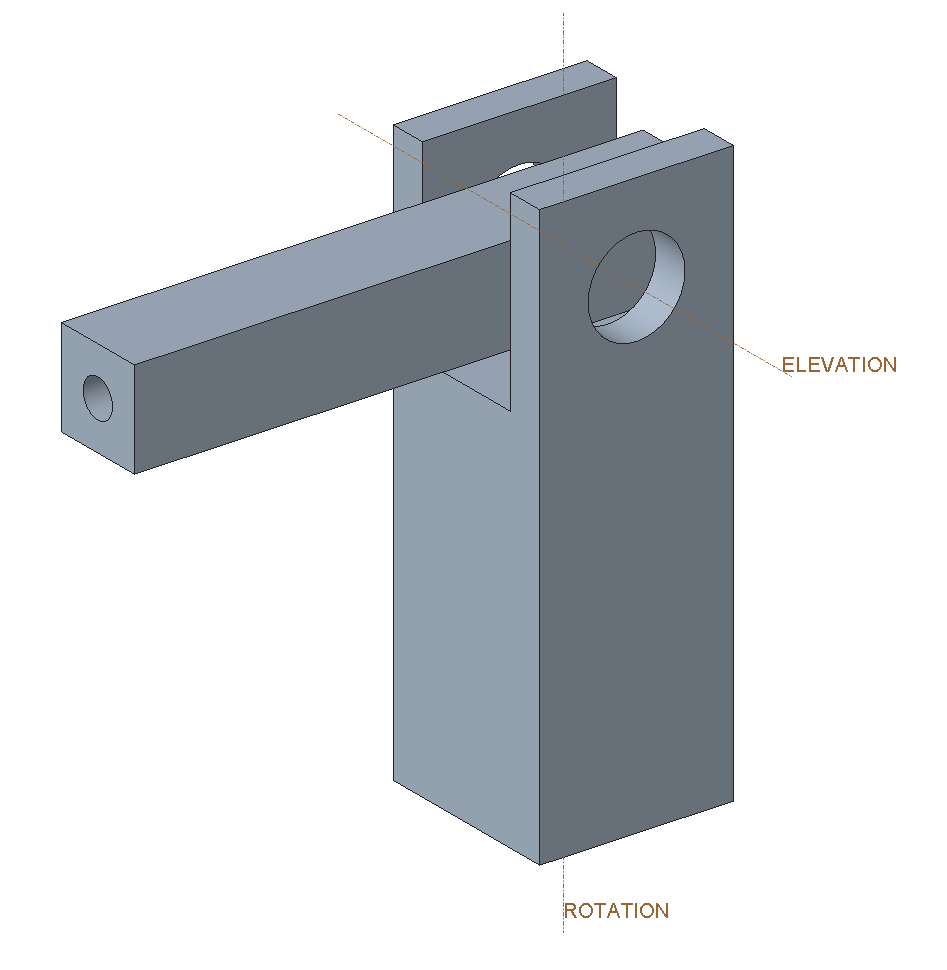
\includegraphics[width=0.6\linewidth]{mockup}
	\caption{A rendszerelrendezés}
	\label{fig:megval_mockup}
\end{figure}

Ki kellett számolnom bizonyos geometriai megkötéseket, amelyek szükségesek a tervezéshez, illetve az alkatrészek kiválasztásához. \\

A torony szükséges fordulatszámát a következőképpen lehet kiszámolni:


\begin{equation}
	rpm_{min} = \frac{v_t}{2 \cdot \pi \cdot r} = \frac{2.778 \w{m/s}}{2 \cdot \pi \cdot \w{m}} = 0.442 \w{1/s} = 26.526 \w{1/min}
\end{equation}

ahol:

\begin{tabular}{cl}
	$v\_t$ & A célpont sebessége a fegyvercsőre merőlegesen, \\
	$r$ & A távolság a célpont és a rendszer között\\
\end{tabular}

Meg lehet állapítani a torony mozgásának felbontását is, tehát hogy hány fokonként lehet állítani a mozgását.

\begin{equation}
	\alpha_{min} = \arcsin\left(\frac{a}{2 \cdot r}\right) \cdot 2 = \arcsin\left(\frac{0.3 \w{m}}{2 \cdot 10 \w{m}}\right) \cdot 2 = 1.719 {^\circ}
\end{equation}

ahol:

\begin{tabular}{cl}
	$a$ & A célpont mérete  \\
	$r$ & A távolság a célpont és a rendszer között\\
\end{tabular}
\pagebreak
\subsection{Mechanikai alkatrészek}
\subsubsection*{Elsütő mechanizmus}
Az elsütő mechanizmusnak egy \textsl{Specna Arms M4}-ből kiszerelt gearbox-ot, illetve annak csövét és hop-up kamráját használtam. A gearbox működése során egy villanymotor több áttételen keresztül hátrahúz egy dugattyút, és azzal együtt a mögötte lévő rugót. Mindeközben a hop-up kamrában betöltődik egy golyó, és megáll a csőben. Ahogy a részlegesen fogazott fogaskerék elengedi a dugattyút, azt a rugó előrelöki, ezáltal a dugattyúkamrában nagy légnyomás keletkezik, ami a fegyver csövén keresztül tud kiegyenlítődni. Folyamatos működés során a motor egymás után húzza fel és engedi el a dugattyút, így amíg van golyó a tárban képes tüzelni. A gearbox belső alkatrészei a \ref{fig:mech_gearboxdiagram}. ábrán láthatóak. 

\begin{figure}[h!]
	\centering
	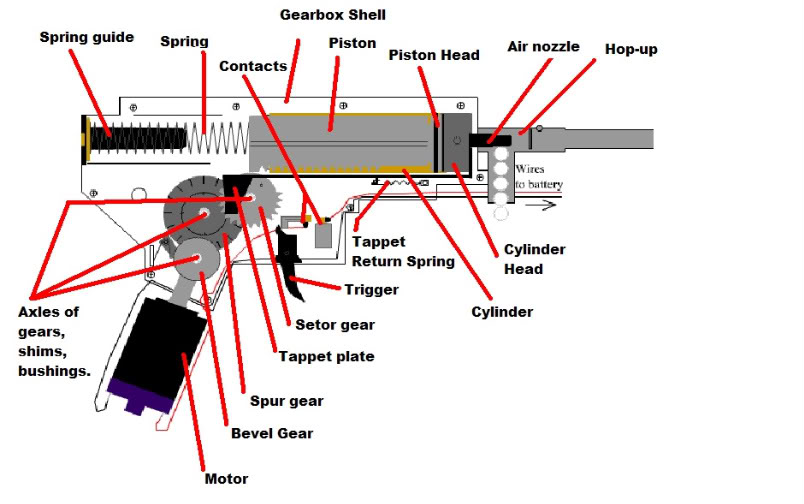
\includegraphics[width=1\linewidth]{mech_gearboxdiagram}
	\caption{V2 gearbox alkatrészei}
	\label{fig:mech_gearboxdiagram}
\end{figure}

A hop-up kamrán belül még található egy gumi csúszófelület, amivel a kilőtt golyó perdületét lehet állítani, ezáltal pedig a fegyver effektív távolságát növelni.

\ABRAKELL

A gearbox-on belül kellett alakítanom a működésen, hogy az előbb leírt folyamatos működést biztosítani tudjam.  Az elsütőbillentyűt, a tűzkapcsolót és minden ehhez tartozó mechanikai elemet kiszereltem, illetve áthuzaloztam. Erre azért volt szükség, mert különben csak a ravasz meghúzásával lehetett volna tüzelni, ami bonyolít a rendszer megvalósításán. A gearbox belső kialakítása a \ref{fig:gearboxbele}. ábrán látható.

\begin{figure}[h!]
	\centering
	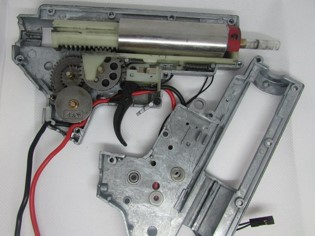
\includegraphics[width=0.6\linewidth]{gearboxbele}
	\caption{A gearbox belseje}
	\label{fig:gearboxbele}
\end{figure}

A fegyver gearbox-ot körülvevő alkatrészeiről le tudtam venni méreteket, ez alapján alakítottam ki később a 3D nyomtatott alkatrészeket. Így végeredményben egy magába zárt alkatrészem lett, amin habár mechanikus nem lehet állítani a tüzelés módját, de csupán két vezetékkel csatlakozik az elektronikához. \\

A gearbox áramfogyasztását illetően találtam méréseket az internet, ahol kifejezetten az én modellemet tesztelték. Az Itteni mérések alapján arra következtettem, hogy 15 A-re méretezni az áramkört megfelelő lehet. \cite{aisroftteszt}

\subsubsection*{Motorok}

A projekthez kettő NEMA-17 léptetőmotort használok\cite{nema17}. Ezek a léptetőmotorok egy széles körben alkalmazott típusa, amelyet főként precíziós mozgatási feladatokhoz használnak, például CNC gépekben, 3D nyomtatókban, robotikai alkalmazásokban és automatizálási rendszerekben. A NEMA-17 esetében a szám a motor elülső oldalának névleges méretét jelenti, amely 1.7 hüvelyk, azaz körülbelül 42,3 mm. A motorok a használt vezérlővel a \ref{fig:mech_stepper}. ábrán láthatóak.\\

\begin{figure}[h!]
	\centering
	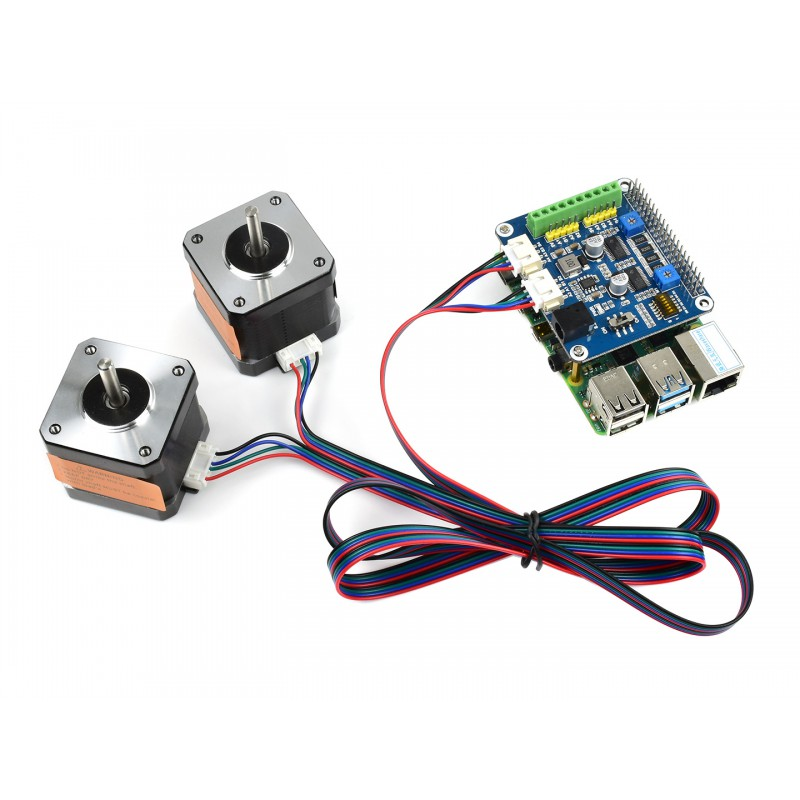
\includegraphics[width=1\linewidth]{mech_stepper}
	\caption{NEMA-17 léptetőmotorok a használt konfigurációban}
	\label{fig:mech_stepper}
\end{figure}

A léptetőmotorok általánosan használt típusai közé tartoznak a szervomotorok és az aszinkron motorok. A léptetőmotorok azonban a mozgásukat apró, egyenlő lépésekre osztják, így lehetővé téve a precíz pozícionálást és sebességszabályozást. A NEMA-17 léptetőmotor tipikusan kétfázisú bipoláris motor, amely négy vezetékes tekercseléssel rendelkezik. Minden lépés során a motor egy adott szöggel fordul el, ami az adott motor típusától és felépítésétől függően tipikusan 1.8 fok, így teljes fordulat esetén 200 lépésre van szükség.\\

Az én esetemben használt léptetőmotorok lépésszöge 1.8 fok, bár ezt a motorvezérlőn lehet tovább osztani. A tartónyomatéka 0.4 Nm. Ezek a paraméterek 10-es áttételű fogaskerék-kapcsolattal megfelelőnek kell lenniük egy ilyen kis teljesítményű alkalmazásnál. 
\subsection{3D tervezés, modellezés}
a
\subsection{Gyártás és összeszerelés}
a
\section{Hardvertervezés}
a
\subsection{Áramköri tervezés}
a
\subsection{Elektronikai alkatrészek}
\subsubsection*{Mikrovezérlő}
A mikrokontroller kiválasztásánál több opciót vizsgáltam, többek között az {Arduino}, az \textsl{STM-32} és a \textsl{Raspberry PI} modelleket. A követelmények a következőek voltak:

\begin{list}{-}{}
	\item Legyen könnyen beszerezhető, mind anyagilag, mind elérhetőség szerint
	\item Megfelelő teljesítmény gépi látás algoritmusokhoz
	\item Elegendő számú GPIO kimenet
	\item Python programozási nyelve támogatása
	\item Ethernet port
\end{list}

Azonban ahogy összehasonlítottam a különböző opciókat, körvonalazódott, hogy a \textsl{Raspberry PI} lesz a megfelelő megoldás. az eszköz a \ref{fig:elek_raspberry4b}. ábrán látható Először is egy gyakorlati szempont szerint, mégpedig hogy egy Raspberry PI 4B modell eredetileg is volt a tulajdonomban 4GB rammal. A gyártó hivatalos fórumán több felhasználó szerint ez már elegendő összetettebb gépi látás algoritmusok futtatására is. \cite{4gbforum} \\

\begin{figure}[h!]
	\centering
	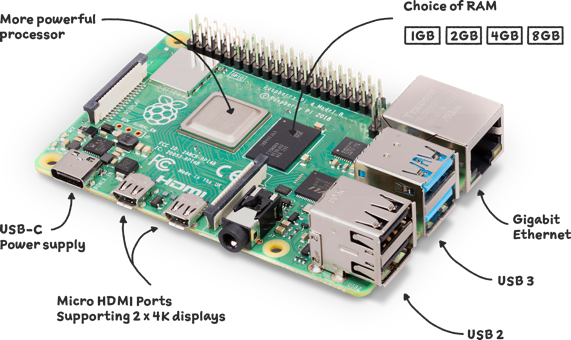
\includegraphics[width=1\linewidth]{elek_raspberry4b}
	\caption{Raspberry 4 model B}
	\label{fig:elek_raspberry4b}
\end{figure}

A kamera illesztése szintén különösen fontos a végtermék működése szempontjából, és ezen a területen magasan kiemelkedik a Raspberry a többi mikrovezérlő közül, mivel magán a gyártó a termékcsaládon belül ajánl több jó minőségű, könnyen beszerezhető kamera modult, amik illesztése már kiforrott az összes Raspberry-hez.\\

Ezentúl a \textsl{Raspberry PI} erősebb, mint a fentebb említett mikrokontrollerek. Linux rendszert futtat, és lehet rajta Python nyelven programozni, ami gépi látás, automatizálás projekteknél hatalmas előny. Számos ki-és bemenete van, ráadásul támogatja a \textsl{Bluetooth}, \textsl{Wi-Fi}, és gigabites \textsl{Ethernet} kapcsolatokat is, nem beszélve a rengeteg bővítő "kabátról", amiket lehet kapni hozzá. Ezek a termék továbbfejlesztését nagyban könnyítik, ráadásul kevesebb munkát kell a nyomtatott áramkör tervezésébe tenni. \cite{raspberry4}

\subsubsection*{Stepper Motor HAT}
A NEMA-17 léptetőmotorok vezérlésére több megoldás is létezik, elterjedtek a \textsl{A4988}, \textsl{TMC5160T} és \textsl{DRV8825} típusú vezérlők. Ezeket azonban vagy külön modulként lehet megvásárolni, vagy pedig SMD alkatrészként, ami mellé mindenképpen kell tervezni kiegészítő áramkört. \\

Azonban a \textsl{Waveshare} cég gyárt egy Raspberry Pi-kompatibilis modult, ami számomra rengeteg segítséget nyújtott. Ez egy külön áramkör, amit a Raspberry GPIO tüskesorára lehet illeszteni. Képes két \textsl{DRV8825} vezérlővel egyszerre kettő léptetőmotort vezérelni. A kártyán lévő kapcsolókkal könnyen lehet állítani külön motoronként a microsteppelést is, amennyiben szükség van rá egészen 1/32-ig. A potméterekkel motoronként tudjuk állítani a maximális felvehető áramot, maximum 2.5 A-ig. A kártyán helyet kapott egy standard 5.5 mm-es csatlakozó is, amivel 8.2 V és 28 V közötti feszültséggel lehet táplálni az áramkört. Egy belső regulator chip segítségével a Raspberry PI-t is el lehet látni árammal, így egy tápegységgel tudom működtetni a teljes áramkört. A modulon több lehetőség is van csatlakoztatni a motorokat, akár sorkapoccsal, akár a léptetőmotorok szabvány csatlakozójával. Ezentúl lehetővé teszi a Raspberry PI GPIO lábainak elérését, csupán arra kell odafigyelni, melyikeket használja. Az eszközről a \ref{fig:elek_stepperhat}. ábrán látható illusztráció. \cite{stepperhat}

\begin{figure}[h!]
	\centering
	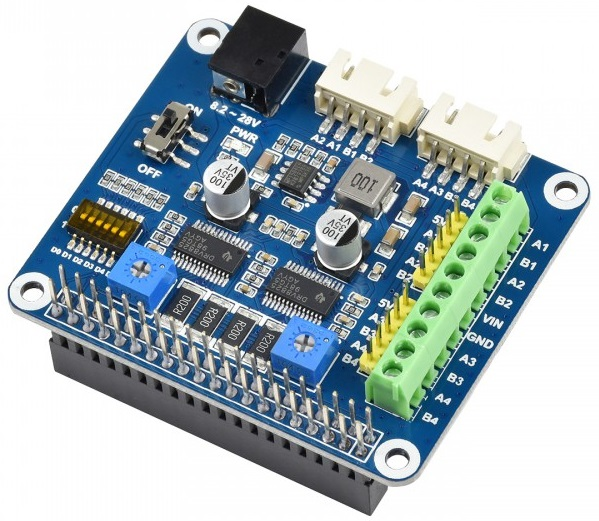
\includegraphics[width=1\linewidth]{elek_stepperhat}
	\caption{Waveshare Stepper HAT}
	\label{fig:elek_stepperhat}
\end{figure}

Az eszköz el lett látva különböző biztonsági funkciókkal, pl. túláram védelemmel, magas hőmérséklet elleni védelemmel, illetve alulfeszültség lockout-tal.\\

A gyártó szintén elérhetővé tett illesztőszoftvereket több eszközre, több motortípusra, amit a későbbiekben én is tudtam használni.

\subsubsection*{Táp}

A prototípust két tápegységről működtetem. Az egyik a Raspberry PI, a léptetőmotorok és a szenzorok áramellátásáért, ez egy standard 5.5 mm-es csatlakozóval ellátott laptop töltő. 14.5 V tápfeszültséget és maximum 5 A áramot képes biztosítani, amely bőven elegendő a vezérlőelektronika ellátására.

\ABRAKELL

A másik táp egy \textsl{HP ps-3701-1} 12 V-os redundáns szervertáp 725 W teljesítménnyel. 

\subsubsection*{Kamera}
A rendszer által használt kamera egy \textsl{Raspberry Pi Camera Module 2} volt.\cite{raspberrycam} Ez a modul 8 MP-es \textsl{Sony IMX219} szenzorral rendelkezik, amivel 3266 x 2450 felbontású állóképet tud készíteni. Képes Full HD videót felvenni 30 fps-el, HD-t 60 fps-el, vagy 640x480 felbontást 90 fps-el. A modul a \ref{fig:elek_raspberrycam}. ábrán látható.

\begin{figure}[h!]
	\centering
	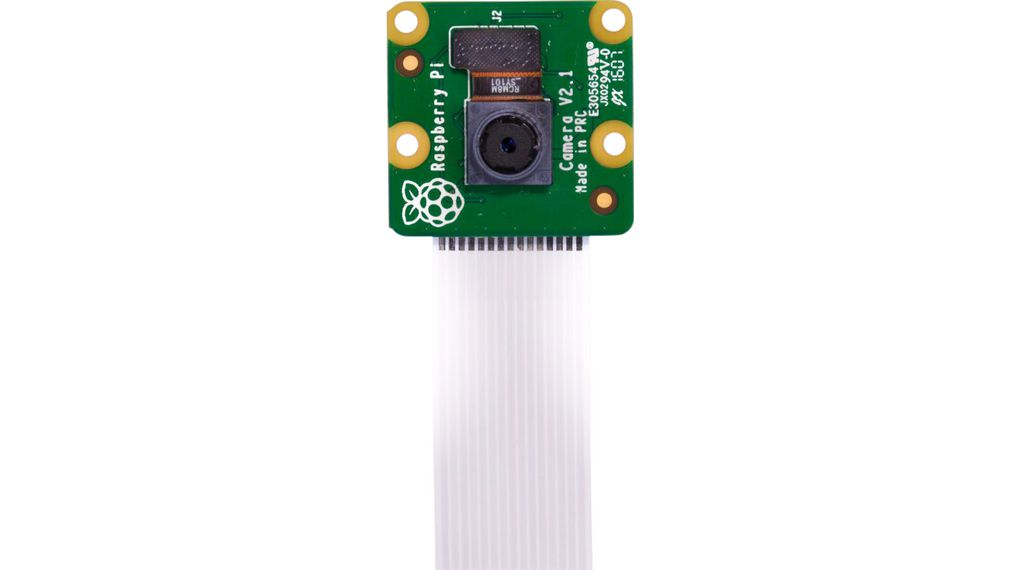
\includegraphics[width=1\linewidth]{elek_raspberrycam}
	\caption{Raspberry Pi Camera Module 2}
	\label{fig:elek_raspberrycam}
\end{figure}

A kamera befoglaló mérete szerelési furatai és CSI portja megegyezik a többi Raspberry kamerával, így a továbbfejlesztés esetén könnyedén lehet őket cserélni.

\subsubsection*{Végálláskapcsoló}
A prototípus bekapcsolásánál fontos, hogy beálljon egy kezdőpozícióba, és ahhoz képest tudjuk viszonyítani a mozgását. Ezt én a két tengelyen 1-1 végálláskapcsolóval oldottam meg. Ezek a modulok könnyen szerelhetőek a 3D nyomtatott vázra, és az alapján adnak jelet, valami van-e az optokapu között. A Raspberry GPIO lábaira könnyedén lehet őket bekötni jumper kábelek segítségével. A szenzorok a \ref{fig:elek_vegallaskapcsolo}. ábrán láthatóak.

\begin{figure}[h!]
	\centering
	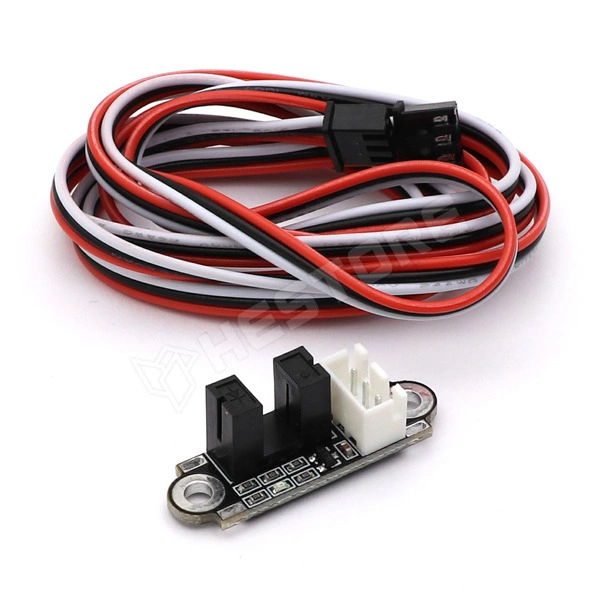
\includegraphics[width=0.5\linewidth]{elek_vegallaskapcsolo}
	\caption{Végálláskapcsoló}
	\label{fig:elek_vegallaskapcsolo}
\end{figure}

\subsection{Hardverintegráció}
a
\subsection{Gyártás, forrasztás}
a
\section{Szoftverfejlesztés}
a
\subsection{Szoftverarchitektúra}
a
\subsection{Adatáramlás, kommunikáció}
a
\subsection{Szinkronizáció?}
a
\subsection{Vezérlő algoritmus}
a
\subsection{Gépi látás}
a
\subsection{Programozási nyelvek és eszközök:}
a
\section{Tesztelés}
a
\subsection{Tesztelési környezet}
a
\subsection{Teljesítménymutatók}
a
\subsection{Kísérleti eredmények}
a
\subsection{Eredmények elemzése}
a
\section{Hibák, észrevételek}
a
\section{Továbbfejlesztési lehetőségek}
a
\section{Költségek}
a
\section{Konklúziók}
a
\section{Köszönetnyilvánítás}
a


\pagebreak
	\begin{thebibliography}{}
	\bibitem{crows}
	Leírás a CROWS rendszerről \hfill (Hozzáférés: 2024.01.22.) \\
	{\footnotesize \url{https://www.globalsecurity.org/military/systems/ground/m101-crows.htm}},
	
	\bibitem{arbalet}
	Leírás az Arbalet-DM rendszerről \hfill (Hozzáférés: 2024.01.22.) \\
	{\footnotesize \url{http://roe.ru/eng/catalog/land-forces/RWS/arbalet-dm/}},
	
	\bibitem{defnder}
	Leírás az deFNder Medium rendszerről \hfill (Hozzáférés: 2024.01.22.) \\
	{\footnotesize \url{https://fnamerica.com/products/weapon-systems/defnder-medium/}},
	
	\bibitem{samsung}
	Leírás a Samsung SGR-A1 rendszerről \hfill (Hozzáférés: 2024.02.10.) \\
	{\footnotesize \url{https://www.globalsecurity.org/military/world/rok/sgr-a1.htm}},
	
	\bibitem{aisroftteszt}
	Teszt az airsoft gearbox áramfogayasztásáról\hfill (Hozzáférés: 2024.10.22.) \\
	{\footnotesize \url{http://www.airsoftlab.eu/docs/experiments/motor_current/}},
	
	\bibitem{nema17}
	A NEMA szabvány\hfill (Hozzáférés: 2024.10.22.) \\
	{\footnotesize \url{https://www.cncitalia.net/file/pdf/nemastandard.pdf}},
	
	\bibitem{4gbforum}
	Felhasználói diskurzus a Raspberry PI gépi látás kapacitásáról\hfill (Hozzáférés: 2024.10.22.) \\
	{\footnotesize \url{https://forums.raspberrypi.com/viewtopic.php?t=366431}},
	
	\bibitem{raspberry4}
	Raspberry 4B specifikációk\hfill (Hozzáférés: 2024.10.22.) \\
	{\footnotesize \url{https://www.raspberrypi.com/products/raspberry-pi-4-model-b/specifications/}},
	
	\bibitem{stepperhat}
	Waveshare stepper motor hat spevifikációk\hfill (Hozzáférés: 2024.10.22.) \\
	{\footnotesize \url{https://www.waveshare.com/wiki/Stepper_Motor_HAT}},

	\bibitem{raspberrycam}
	Raspberry 2 kamera specifikációk\hfill (Hozzáférés: 2024.10.22.) \\
	{\footnotesize \url{https://www.raspberrypi.com/products/camera-module-v2/}},

\end{thebibliography}


\end{document}